\section{Basic concepts} 
\label{sec:Basics}
Action potentials and extracellular potentials are electric signals, and to understand them, we need to have some basic knowledge about the physics of electricity. 


\subsection{\orange{GH: Electric charge}}
The fundamental quantity for electricity is the charge carried by the protons and electrons that build up the atoms that build up the material world. The proton has a charge $e$, while the electron has a charge $-e$, where $e = 1.602\times10^{-19}$ Coulomb (C) is the unit charge. 

In the brain, the charge carriers are not free electrons (or protons), but ions. Ions are atoms or molecules that have gained or donated one or several electrons, and therefore have become electrically charged. Important charge carriers in the brain are sodium and potassium ions (Na$^+$ and K$^+$ with charge $1e$), chloride ions (Cl$^-$ with charge $-1e$, and calcium ions (Ca$^{2+}$ with charge $2e$), which are floating around in the saline solutions that fill both the intracellular and extracellular space.

Starting at a fundamental level, a pair of charges, $q'$ and $q$, will act on each others with a force given by Coulomb's law:

\begin{equation}
F = k_e\frac{q q'}{r^2}, 
\label{Basics:eq:CoulombF}
\end{equation}
where $k_e = 8.99\times10^9$ N$\cdot$ m$^2\cdot$C$^{-2}$ is Coulomb's constant, and $r$ is the distance between the two charges. The direction of the force is along the line between the two charges, and the force will be repelling if the charges have the same valency (sign) and attractive if they have the opposite valency. 

If there are several point charges present, the contribution from each of them sum up linearly. We can then use Coulomb's law to compute the net force that will act on one charge $q$ in a position ${\bf r}$, by summing the contributions from all other charges $q_1, q_2, q_3 ... q_N$ in positions ${\bf r_1}, {\bf r_2}, {\bf r_3} ... {\bf r_N}$: 
\begin{equation}
{\bf F}({\bf r}) = \sum_{n=1}^N k_e q q_n \frac{{\bf r}-{\bf r_n}}{|{\bf r}-{\bf r_n}|^3}.
\label{Basics:eq:CoulombFN}
\end{equation}
We have here used a boldface notation to indicate that the force and positions are vectors, entities that have both a magnitude and spatial direction. The position vector ${\bf r}$ can be visualized as an arrow from a reference point $r=0$ to the position of the charge $q$. Likewise, the vector ${\bf r}-{\bf r_n}$ as an arrow between the positions of the charge pair $q$ and $q_n$, defining both the distance and direction of the (imagined) line connecting them.

If our system of study consisted of a small number $N_{small}$ of charges, we could use $N_{small}$ instances of eq. \ref{Basics:eq:CoulombFN} to compute the force acting on each individual charge. Together with Newton's law ${\bf F} = m {\bf a}$, which tells us how the charges will be accelerated in the force direction, eq.\ref{Basics:eq:CoulombFN} would then allow us to compute the movements of all our charges over time. However, when trying to understand what is going on in the brain, we are usually not interested such microscopic interactions between a small number of charges, but rather the joint interactions of a very, very large number of particles. It is then not feasible to keep track of the motion of each individual charge. 

At the larger scale, it is therefore more useful to work with electric fields, which we will define below. It is still nice to have taken a look at  Eq. \ref{Basics:eq:CoulombFN}, since it establishes the fundamental origin of electrical forces and fields. 


\subsection{\orange{GH: Electric fields}}
The electric field at a given location (measured in volts per meter (V/m)) can be defined as the force that will act on a reference charge $q$ present there, i.e., 
\begin{equation}
{\bf E}({\bf r}) = {\bf F}({\bf r})/q.
\label{Basics:eq:E}
\end{equation}
If we assume that this force is exclusively due to the Coulomb interaction between electric charges, the electric field can be obtained by inserting eq. \ref{Basics:eq:CoulombFN} into eq. \ref{Basics:eq:E}:
\begin{equation}
{\bf E}({\bf r}) = \sum_{n=1}^N k_e q_n \frac{{\bf r}-{\bf r_n}}{|{\bf r}-{\bf r_n}|^3}.
\label{Basics:eq:CoulombEN}
\end{equation}

Eq. \ref{Basics:eq:CoulombEN} applies to a microscopic level, and varies with a very fine spatial resolution. For example, it will be big at locations that are close to an individual charge (i.e., where $|{\bf r}-{\bf r_n}|$ for some $n$ is small), and smaller at points where the distance to the nearest charge is longer. A direct use of eq. \ref{Basics:eq:CoulombEN} will therefore force us to keep track of each individual charge, and as we argued in the previous subsection, this is not a feasible when we want to study a macroscopic system. Eq.\ref{Basics:eq:CoulombEN} is therefore not very useful for us.

Fortunately, microscopic field variations are not what we are interested in when we are trying to understand the brain. A technical argument for why this is not the case, is that the electrodes used for recording brain signals have a tip diameter on the order of a micrometer or so, which is much, much larger than the average intra-charge distance in the saline solution of the brain. The electrodes therefore do not "see" the microscopic fluctuations, but rather record an average taken over the electrode surface. When we speak of an electric field or potential in the brain, we therefore always mean field or potential on a so-called \textit{coarse-grained} scale, averaged over an electrode surface of at least $1 \mu$m$^2$. A non-technical argument is that it is this coarse-grained signal, and not the microscopic reality that is bubbling underneath it, that are of importance if we want to understand the key brain processes. 

From here on, we shall not think of ${\bf E}$ as something that we compute based on
knowledge of the microscopic charge distribution (cf. eg. \ref{Basics:eq:CoulombEN}), but rather as a higher level entity, exerting an average force on charges in a certain direction.


\subsection{\orange{GH: Electric potentials}}
Tightly related to the electric field ${\bf E}$ is the electric potential $\phi$ (with units volt (V)), which is what we normally measure experimentally when we stick an electrode into the brain. While ${\bf E}$ is a fundamental physical entity, $\phi$ may be regarded as an auxiliary variable. It is a way to represent the electric field that often makes computations simpler, and measurements easier. 

In the quasi-electrostatic regime, the electric field can be expressed as the spatial derivative, or gradient, of the potential:
\begin{equation}
{\bf E}(x,y,z) = - \nabla \phi(x,y,z) = - \left(\frac{d\phi}{dx} {\bf e_x}  + \frac{d\phi}{dy} {\bf e_y} + \frac{d\phi}{dz} {\bf e_z} \right) \phi.
\label{Basics:eq:EV}
\end{equation}
The operator $\nabla$ computes a property's spatial rate of change in the various spatial directions, and ${\bf e_x}$, ${\bf e_y}$ and  ${\bf e_z}$ are the unit vectors in the three spatial directions $x$, $y$ and $z$, respectively. Unlike ${\bf E}$, which is a vector-field, $\phi$ is a scalar function, and as such, it tends to be easier to deal with.

To get an intuitive understanding of the relationship between ${\bf E}$ and $\phi$, it helps to consider an idealized one-dimensional scenario with a constant field in the $x$-direction. Then, eq. \ref{Basics:eq:EV} simplifies to,
\begin{equation}
E = -\frac{d\phi(x)}{dx} = -\frac{\Delta \phi}{\Delta x} = -\frac{\phi(x_b)-\phi(x_a)}{x_b-x_a},
\label{Basics:eq:EV1D}
\end{equation}
where the first equality follows from the 1D-assumption, the second from the assumption that $E$ is constant, and the third is simply a definition of the second, where $x_b$ and $x_a$ may represent any two arbitrary points in space. For example, if $E = 1$ V/m, and if the distance between our points $x_b-x_a$ is 1m, Eq. \ref{Basics:eq:EV1D} tells us that $\phi$ will be 1 V  lower in $x_b$ compared to $x_a$ (Fig. \ref{Basics:fig:Ground}).

\begin{figure}[!ht]
\begin{center}
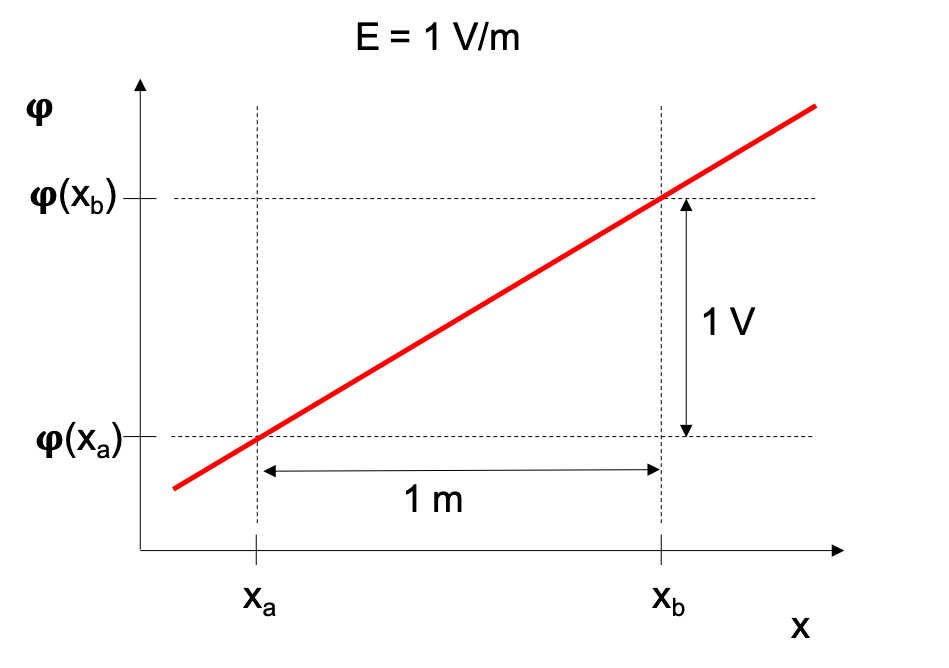
\includegraphics[width=0.8\textwidth]{Figures/Basics/Ground.png}
\end{center}
\caption{\textbf{Relationship between the electric field and electric potential.} With a constant electric field $E = 1$ V/m, the electric potential $\phi$ increases linearly with distance $x$. With two locations $x_a$ and $x_b$ 1 m apart, we know that $\phi(x_b) = \phi(x_a) + 1$ V. We are free to define an arbitrary reference point (ground) for the $\phi$, and if we take $\phi(x_a) = 0$, it follows that $\phi(x) = (x-x_a) \times E$. In $x_b$, we then get $\phi(x_b)=$(1m)$\times$1V/m$=1$V.
}
\label{Basics:fig:Ground}
\end{figure}

Based on the last example, we also would like to make a comment on \textit{grounding}. The field ${\bf E}$ generally determines the potential only up to a constant. In the example, the field $E = 1$ V/m would be consistent with any pair of potentials $\phi_a$ and $\phi_b$ as long as $\phi_b = \phi_a + 1$ V. Since it is the field (not the potential) that is the fundamental physical entity, we can therefore not speak of the potential in a certain point as an absolute entity, but only of the potential \textit{difference} between two points. When we record potential in a given location, we therefore always record it relative to some an arbitrary reference point, which we normally call \textit{ground}, and where we define $\phi = 0$ (cf. example in Fig. \ref{Basics:fig:Ground}). 

When recording extracellular potential, the reference electrode can be placed either outside or inside brain tissue \cite{Sharott2015}, but typically sufficiently far away that one can assume that the potential at the reference electrode is not affected by the processes that one wishes to investigate with the measuring electrode. 

The unit (V) of the electric potential is equivalent to energy per charge, or Joule per Coulomb (V = J/C). The electric potential can therefore be defined as the energy needed to move a unit of electric charge $q$ from the reference point (ground) to a specific location. As such, the concept of an electric potential is closely related to the concept of a potential energy. The potential energy ($U_E$) of a charge $q$ in an electric field is:
\begin{equation}
U_E = q\phi.
\label{Basics:eq:UE}
\end{equation}


\subsection{\orange{GH: Electric current}}
When studying the brain, we do not track individual charges, but are rather interested in the net movement of charge at a coarse-grained (space averaged) scale. In an electrical cable, such as those powering a lamp in a normal house, the total movement of charge (through the one-dimensional the cable) is normally described in terms of an electrical current ${\bf I}$, with units Ampere (A = C/s). For currents in a three dimensional volume, such as brain tissue, it is more convenient to work with current densities, ${\bf i}$ (A/(m$^2$)), which is defined as the current per unit cross section area. 

Before defining the current density further, we need to say some words about the medium that it runs through. Neural membranes are largely dielectric in their nature. In a dielectric medium, charges are bound to stay in confined regions of space, and an electric field only will slightly shift their average equilibrium positions, causing a polarization of the material. It is such a polarization that gives rise to the neuronal membrane potential. 

Unlike the dielectric membrane, the saline solution that fill up the intra- and extracellular space is predominantly of conductive nature, which means that charges move rather freely through it when exposed to an electric field. As currents that pass through brain tissue predominantly move through the extracellular part of it, we shall represent the tissue as a conductor. 

For most parts of this book, we shall approximate brain tissue as a \textit{linear} conductor, which means that the current densities are given by the formula:
\begin{equation}
{\bf i} = \sigma {\bf E}, 
\label{Basics:eq:i}
\end{equation}
which is a version of Ohm's law. It states that the current density will be proportional to the electric field and the conductivity of the medium, $\sigma$, which has units Siemens per square meters (S/m$^2$). The conductivity is a material property, and in brain tissue, it is often assumed to be a constant, at least within a given brain region. 

It is important to point out that the current given by eq. \ref{Basics:eq:i} represents the average movement on charge on a coarse-grained level, and does not apply on a microscopic scale. If we compare it with the microscopic fundament for this movement, it is easy to get confused, so let us enter that confusion and try to clear it up. According to eq. \ref{Basics:eq:E}, an electric field will act on a reference charge $q$ by a constant force, which according to Newton's law (${\bf F} = m{\bf a}$) should give it a constant acceleration in the field-direction. Conversely, eq. \ref{Basics:eq:i} states that ${\bf E}$ gives rise, not to a constant acceleration of charges, but rather a constant current, i.e., a constant average \textit{velocity} of charges. 

The reason for the discrepancy between the microscopic (constant acceleration) and macroscopic (constant velocity) level is that the constant acceleration (eq. \ref{Basics:eq:E}) at the microscopic level will go on for only a very very tiny time period (called the charge relaxation-time) \index{Charge-relaxation} before our protagonist charge $q$ will bump into some other particle and be scattered out in some random direction. After the scattering event, the acceleration will start "from scratch" again, and go on until the next collision takes place, and so on. Whereas the scattering events will tend to make the motion of $q$ a random walk (which should give it a zero average velocity in any preferred direction), the small periods of acceleration between collisions will at average give $q$ a net drift velocity in the field direction. As the same will happen for all other charges present, there will be a net drift of charge in the field direction. This (average) drift happens to depend linearly on the field, and constitutes the current density given by Eq. \ref{Basics:eq:i}, which is often referred to as the drift current density. The fact that this relationship is linear (constant velocity) is constitutive, meaning that it is observed experimentally rather than derived from first physical principles \citep{Nunez2006, Pettersen2012}.


\subsection{\orange{GH: Electroneutrality of brain tissue}}
Due to the Coulomb force (eq. \ref{Basics:eq:CoulombF}), positive charges will repel other positive charges, and attract negative charges. The effect of this is that the charges in a medium will  arrange themselves so that the numbers of positive and negative charges in a finite volume of space tends to be equal. For this reason, any reference volume of brain tissue will, on the coarse-grained scale, be practically electroneutral \cite{Nunez2006, Grodzinsky2011}. If this were not the case, and a volume did contain a net charge density $\rho$, the very strong Coulomb-forces associated with it would cause $\rho$ to decay to zero at a rate proportional to the so-called \textit{charge-relaxation time}, which in brain tissue is in the order of a nanosecond \cite{Grodzinsky2011}. 

The Coulomb force also gives rise to a phenomenon called Debye shielding \cite{Nunez2006}. As opposites attract, positive charges will tend to surround themselves with negative charges, and vice versa. The equally numbered positive and negative charges in a reference volume will in that way tend to shield (cancel out) the electric fields from one another, so that neither of them give any contribution to the field measured at some distance away from the charges.

Of course, a non-zero electric field or potential does require some charge separation somewhere. In the brain, this predominantly happens in at neuronal membranes, and on a very small spatial scale. Working as a parallel plate capacitor, a patch of membrane separates a charge $Q$ on the interior side from a charge $-Q$ on the exterior side. These two charges are equal in magnitude and opposite in sign, and are distributed in nanometer-thick sheaths on the interior and exterior membrane, called Debye layers. This charge separation gives rise to the membrane potential $V_m = Q/C_m$, where $C_m$ is the capacitance (with units Fahrad (F)) of the patch of membrane. We will speak more of the membrane capacitance in Chapter \ref{sec:Neuron}, but the point that we wanted to make here is that, since the membrane is just some nanometers thick, the two charges $-Q$ and $Q$ are very close in space, and will shield each others' contributions to measured extracellular fields since these, again, are space-averages over micrometer-regions.

The practical implication of electroneutrality and shielding effects is that, when we study extracellular potentials (or fields), we can neglect contributions from any particular distribution of charges, and instead compute extracellular potentials from the constraint that there should be no charge accumulation anywhere in the extracellular space. As we shall elaborate on in Chapter \ref{sec:VC}, the sources for the extracellular potential (of field) will then exclusively be the currents entering or leaving the extracellular space through neural membranes. Mathematically, we can express this by the continuity equation:
\begin{equation}
\nabla \cdot {\bf i} = -C.
\label{Basics:eq:continuity1}
\end{equation}
where the source term, $C$, is called the current source density (units A/m$^3$), and represents the transmembrane output currents from neurons. 

Eq. \ref{Basics:eq:continuity1} tells us that at in a volume of space where there is no neuronal membrane ($C = 0$), we have that $\nabla \cdot {\bf i} = 0$. This means that there will be no net extracellular current entering or leaving such a volume. In a volume that does receive a neuronal output, eq. \ref{Basics:eq:continuity1} tells us that the current outputted from the neuron into that volume must be carried away from that volume as an extracellular current. As we shall show in Chapter \ref{sec:VC}, this conservation law shall be the fundament for modeling extracellular potentials surrounding active neurons.

\ghnote{GH: Maybe a figure here, showing current-loops.}


\subsection{\orange{GH: Maxwell's equations}}
We could have started this chapter on introductory theory by listing up Maxwell's equations, since they are the fundament for most of the physics that we have gone through so far. However, since they may appear a bit challenging for "the untrained eye", we chose a "softer" path, which, although it is rather incomplete, we deemed sufficient for establishing the main concept that we will use in the remainder of this book. 

For good taste, we still wanted include Maxwell's equations, and list them here for later reference. The equations come in two versions, referred to as the microscopic and macroscopic versions. The microscopic version is the most fundamental, but using it requires knowledge of the positions of all individual charges, which is unfeasible when we study brain tissue or any other medium at a macroscopic level. We therefore only list up the macroscopic set of equations: 

\begin{eqnarray}
\nabla\cdot {\bf D} & = & \rho. \label{Basics:eq:Max1} \\
\nabla \cdot {\bf B} & = & 0.  \label{Basics:eq:Max2} \\
\nabla \times {\bf E} & = & - \frac{\partial {\bf B}}{\partial t}.  \label{Basics:eq:Max3} \\
\nabla \times {\bf H} & = & \bf{i} + \frac{\partial {\bf D}}{\partial t}.  \label{Basics:eq:Max4}
\label{Basics:eq:Maxwell}
\end{eqnarray}

Eq. \ref{Basics:eq:Max1} is called Gauss's law (for electricity). The variable ${\bf D}$ is called the \textit{displacement field}, and $\rho$ is the free (unbound) charge density, which generally can be non-zero, although we argued earlier that brain tissue for practical purposes can be assumed to be electroneutral at the coarse-grained scale. ${\bf D}$ is tightly related to the total electric field ${\bf E}$ that we have introduced earlier. In a linear dielectric medium (and we will in this book assume that our mediums are linear), it holds that ${\bf D} = \epsilon {\bf E}$, where $\epsilon$ is the electric permittivity of the medium. 

Eq. \ref{Basics:eq:Max2} is Gauss's law for magnetism, and is the magnetic equivalent to eq. \ref{Basics:eq:Max1}, with {\bf B} being the magnetic induction field.  Whereas eq. \ref{Basics:eq:Max1} states that there can be spatial gradient of the electric field due to a local charge density $\rho$, eq. \ref{Basics:eq:Max1} disallows the corresponding gradient in the magnetic induction field, simply because magnetic monopoles do not exist. 

Eq. \ref{Basics:eq:Max3} is the Maxwell-Faraday equation for electric induction. The cross product $\nabla \times {\bf E}$ represents a certain kind of change in the electric field called the \textit{curl}. The equation tells us that such a change will be induced if there is a temporal variation in the magnetic induction field. 

Eq.  \ref{Basics:eq:Max4} is Ampere's circuital law, and is the magnetic equivalent to eq. \ref{Basics:eq:Max3}. Here, the magnetic field ${\bf H}$ is related to the magnetic induction field ${\bf B}$ in a way equivalent to how the electric field ${\bf E}$ is related to the displacement field ${\bf D}$, and in a linear medium, ${\bf B} = \mu{\bf H}$, with the proportionality constant $\mu$ being the magnetic permeability of the medium. According to eq. \ref{Basics:eq:Max4}, a magnetic field will be induced either by an electric current going through the medium (first term on the right), or by a temporal change in the displacement field (second term on the right). 

Together, eq. \ref{Basics:eq:Max1} and \ref{Basics:eq:Max3} show that an electric field can originate either from electric charges, or from time-varying magnetic fields. However, for brain tissue, we shall assume that the quasi-static approximation of Maxwell's equations are warranted, which means that the terms with temporal derivatives of the electric and magnetic fields are neglected in eqns. \ref{Basics:eq:Max3} and  \ref{Basics:eq:Max4}. This assumption was implicit when we earlier expressed {\bf E} as a function of charges in eq. \ref{Basics:eq:CoulombEN}. In the quasi-static case we also get from eq. \ref{Basics:eq:Max3} that $\nabla \times {\bf E} = 0$, which is a prerequisite for expressing ${\bf E}$ as a gradient of a potential (cf. eq. \ref{Basics:eq:EV}). For the magnetic field, we get from eq. \ref{Basics:eq:Max4} that $\nabla \times {\bf H} = \bf{i}$. This allows us to predict magnetic fields from electric tissue currents, and is the fundamental relation for interpreting magetoencephalohy data (see Chapter \ref{sec:MEG}).

Also the concept of charge conservation follows from Maxwell's equations. We can see this if we 
compute the divergence (take $\nabla \cdot$) of both sides of \ref{Basics:eq:Max4}:
\begin{equation}
- \nabla \cdot \bf{i} =  \frac{\partial {\bf \nabla \cdot D}}{\partial t}, 
\label{Basics:eq:Max4dot}
\end{equation}
and insert \ref{Basics:eq:Max1} on the right hand side, to get:
\begin{equation}
- \nabla \cdot \bf{i} =  \frac{\partial \rho}{\partial t},
\label{Basics:eq:Max4dot1}
\end{equation}
If the left hand side in nonzero, it means that there will be a net influx of current into a volume, and if that is the case, we must have an accumulation of charge there, as described by the right hand side of the equation. In the case of electroneutrality ($\rho = 0$), eq. \ref{Basics:eq:Max4dot1} reduces to the earlier postulated eq. \ref{Basics:eq:continuity1}, but without the source term. 

The rationale behind the source term in eq. \ref{Basics:eq:continuity1} is that the transmembrane source currents are not accounted for in the current density $\bf{i}$, since we in this book shall use it to model only extracellular currents. The transmembrane currents will therefore appear as an external input to our extracellular system. 



